% --------------------------------------------------------------------------------

\begin{exercise}

Sei $A \in \R^{2 \times 2}$ eine symmetrische, positiv definite Matrix, $b \in \R^2$ und $c > 0$ mit $c - \frac{1}{2}\Div(b) \geq 0$.
Weiter seien $\Omega \subset \R^2$ ein beschränktes Lipschitz-Gebiet und $f \in L^2(\Omega)$.

\begin{enumerate}[label = \textbf{\alph*)}]

  \item Beweisen Sie, dass eine eindeutige schwache Lösung $u \in H_0^1(\Omega)$ von

  \begin{subequations}
    \begin{align}
      -\Div(A\nabla u) + b \cdot \nabla u + cu &= f \qquad \text{auf } \Omega, \label{eq:1A} \\
      u &= 0 \qquad \text{auf } \partial\Omega, \label{eq:1B}
    \end{align}
  \end{subequations}

  existiert.

  \item Sei $u_h \in \mathcal{S}_0^1(\mathcal{T})$ die eindeutige, schwache Finite-Elemente Lösung.
  Konstruieren Sie einen residualen Fehlerschätzer für
  $\norm[H_0^1(\Omega)]{u - u_h}$.

  \item Beweisen Sie, dass dieser Fehlerschätzer zuverlässig ist.

\end{enumerate}

\textit{Hinweis:}
Zeigen Sie zuerst, dass die zugehörige Bilinearform elliptisch ist.

\end{exercise}

% --------------------------------------------------------------------------------

\begin{solution}

Wir stellen zuerst das Funktional und die Bilinearform für die schwache Formulierung der PDE (1) auf.
$\Forall v \in H_0^1(\Omega):$

\begin{align*}
  F(v)
  & :=
  \Int[\Omega]{f v}{x}
  \stackrel{!}{=}
  \Int[\Omega]{(-\Div(A \nabla u) + b \cdot \nabla u + c u) v}{x}
  =
  -\Int[\Omega]{\Div(A \nabla u) v}{x}
  +
  \Int[\Omega]{(b \cdot \nabla u + c u) v}{x} \\
  & \stackrel
  {
    \mathrm{PI}
  }{=}
  \Int[\Omega]{A \nabla u \cdot \nabla v}{x}
  -
  \underbrace
  {
    \Int[\partial \Omega]{(A \nabla u \cdot \nu) v}{s}
  }_{=0}
  +
  \Int[\Omega]{(b \cdot \nabla u + c u) v}{x}
  =
  \Int[\Omega]{(\nabla u, \nabla v)_A + (b \cdot \nabla u + c u) v}{x} \\
  & =:
  a(u, v)
\end{align*}

Weil $\R^2$ endlich-dimensional ist, ist die, wegen der Symmetrie und positiven Definitheit von $A$ wohldefinierte, Energie-Norm $\norm[A]{\cdot}$ äquivalent zur Euklid-Norm $|\cdot|$.

\begin{align*}
  \implies
  \Exists \alpha, \beta > 0:
  \alpha |\cdot| \leq \norm[A]{\cdot} \leq \beta |\cdot|
\end{align*}

\begin{enumerate}[label = \textbf{\alph*)}]

  \item Wir wollen Exercise 7 (Lemma of Lax-Milgram) auf $F, a$ und $H_0^1(\Omega)$ anwenden.

  \begin{enumerate}[label = \arabic*.]

    \item $a$ stetig: Wir nehmen zusätzlich $b \in L^{\infty}(\Omega)$ an.

    \begin{align*}
      a(u, v)
      & =
      \Int[\Omega]{(\nabla u, \nabla v)_A + (b \cdot \nabla u + c u) v}{x}
      \stackrel
      {
        \mathrm{CSB}
      }{\leq}
      \Int[\Omega]{\norm[A]{\nabla u} \norm[A]{\nabla v} + |b| |\nabla u| v + c u v}{x} \\
      & \leq
      \beta^2 \Int[\Omega]{|\nabla u| |\nabla v|}{x}
      +
      \norm[L^\infty]{b} \Int[\Omega]{|\nabla u| |v|}{x}
      +
      c \Int[\Omega]{u v}{x} \\
      &\stackrel
      {
        \mathrm{CSB}
      }{
      \leq}
      \beta^2 \norm[L^2(\Omega)]{\nabla u} \norm[L^2(\Omega)]{\nabla v}
      +
      \norm[L^\infty(\Omega)]{b} \norm[L^2(\Omega)]{\nabla u} \norm[L^2(\Omega)]{v}
      +
      c \norm[L^2(\Omega)]{u} \norm[L^2(\Omega)]{v} \\
      & \leq
      \max \Bbraces{\beta^2, \norm[L^\infty(\Omega)]{b}, c} \norm[H^1(\Omega)]{u} \norm[H^1(\Omega)]{v}
    \end{align*}

    \item $a$ elliptisch:

    Die Produktregel für $\Div$ liefert uns

    \begin{align*}
      \Div(u^2 b) = \nabla(u^2) b + u^2 \Div b = 2 u b \nabla u + u^2 \Div b
      \implies
      u b \cdot \nabla u = \frac{1}{2} (\Div(u^2 b) - u^2 \Div b),
    \end{align*}

    und der Integral-Satz von Gauß, dass ($u \in H_0^1(\Omega)$)

    \begin{align*}
      \Int[\Omega]{\Div (u^2 b)}{x}
      =
      \Int[\partial \Omega]{u^2 b \cdot \nu}{s}
      =
      0.
    \end{align*}

    Wir verwenden die Poincaré-Ungleichung.

    \includegraphicsboxed{PDEs/PDEs_-_Satz_5-11_(Poincare-Ungleichung).png}

    \begin{align*}
      \implies
      a(u, u)
      & =
      \Int[\Omega]{(\nabla u, \nabla u)_A + (b \cdot \nabla u + c u) u}{x}
      =
      \Int[\Omega]{\norm[A]{\nabla u}^2 + u b \cdot \nabla u + c u^2}{x} \\
      & \geq
      \Int[\Omega]{\alpha^2 |\nabla u|^2 + \frac{1}{2} (\Div(u^2 b) - u^2 \Div b) + c u^2}{x} \\
      & =
      \alpha^2 \norm[L^2(\Omega)]{\nabla u}^2
      +
      \frac{1}{2} \underbrace{\Int[\partial \Omega]{u^2 b \cdot \nu}{s}}_{=0}
      +
      \underbrace
      {
        \Int[\Omega]{\pbraces{c - \frac{1}{2} \Div b} u^2}{x}
      }_{
        \geq 0
      } \\
      & \geq
      \alpha^2 \norm[L^2(\Omega)]{\nabla u}^2
      \geq
      \frac{\alpha^2}{C_P^2 + 1} \norm[H^1(\Omega)]{u}^2
    \end{align*}

  \end{enumerate}

  \item Siehe \textbf{c)} ...

  \item Wir formulieren ein Analogon zu Theorem 4.11.

  \includegraphicsboxed{NumPDEs/NumPDEs - Theorem 4.11.png}

  \begin{tcolorbox}[standard jigsaw, opacityback = 0]
    \textbf{Theorem 4.11. (Hier könnte Ihre Werbung stehen!)}
    Der Fehlerschätzer

    \begin{align*}
      \eta
      :=
      \pbraces
      {
        \norm[L^2(\Omega)]{h_\mathcal{T} (f - b \cdot \nabla u_h - c u_h)}^2
        +
        \norm[L^2(\mathcal{E}_\Omega)]{h_\mathcal{E}^{1/2} \dbbraces{\partial_n (A u_h)}}^2
      }^{1/2}
    \end{align*}

    genügt der Zuverlässigkeits-Abschätzung

    \begin{align*}
      \norm[H^1(\Omega)]{u - u_h}
      \leq
      C \eta,
    \end{align*}

    wobei die Konstante $C > 0$ von der $\gamma$-Form-Regularität von $\mathcal{T}$ abhängt.

  \end{tcolorbox}

  \textbf{Beweis.}
  Für alle $w \in H_D^1(\Omega)$ und $T \in \mathcal{T}$, führt partielle Integration, und die Tatsache, dass $u_h \in \mathcal{S}^1(\Omega)$ und $A$ konstant ist, zu

  \begin{multline*}
    \Int[T]{(\nabla u_h, \nabla w)_A + (b \cdot \nabla u_h + c u_h) w}{x}
    =
    \Int[T]{A \nabla u_h \cdot \nabla w}{x}
    +
    \Int[T]{(b \cdot \nabla u_h + c u_h) w}{x} \\
    \stackrel
    {
      \mathrm{PI}
    }{=}
    -\Int[T]
    {
      \underbrace
      {
        \Div(A \nabla u_h)
      }_{=0}
      w
    }{x}
    +
    \Int[\partial T]{\partial_n(A u_h) w}{s}
    +
    \Int[T]{(b \cdot \nabla u_h + c u_h) w}{x}.
  \end{multline*}

  Wir erinnern uns an die Definition vom \enquote{Sprung der Normalen-Ableitung}.

  \includegraphicsboxed{NumPDEs/NumPDEs - (4.34).png}

  Wir betrachten das Residuum $R_h \in H_0^1(\Omega)^*$:
  \begin{align*}
    \implies
    R_h(w)
    & :=
    F(w) - a(u_h, w)
    =
    (f; w)_{L^2(\Omega)}
    -
    \sum_{T \in \mathcal{T}}
    \Int[T]{(\nabla u_h, \nabla w)_A + (b \cdot \nabla u_h + c u_h) w}{x} \\
    & =
    (f - b \cdot \nabla u_h - c u_h; w)_{L^2(\Omega)}
    -
    \sum_{T \in \mathcal{T}}
    (\partial_n (A u_h); w)_{L^2(\partial T)} \\
    & =
    \sum_{T \in \mathcal{T}}
    (f - b \cdot \nabla u_h - c u_h; w)_{L^2(T)}
    -
    \underbrace
    {
      \sum_{E \in \mathcal{E}_D}
      (\partial_{n_E^-} (A u_h); w)_{L^2(E)}
    }_0
    -
    \sum_{E \in \mathcal{E}_\Omega}
    (\dbbraces{\partial_n (A u_h)}_E; w)_{L^2(E)} \\
    & \stackrel
    {
      \mathrm{CSB}
    }{\leq}
    \sum_{T \in \mathcal{T}}
    \norm[L^2(T)]{f - b \cdot \nabla u_h - c u_h}
    \norm[L^2(T)]{w}
    +
    \sum_{E \in \mathcal{E}_\Omega}
    \norm[L^2(E)]{\dbbraces{\partial_n(A u_h)}_E}
    \norm[L^2(E)]{w}
  \end{align*}

  Für beliebiges $v \in H_D^1(\Omega)$, wählen wir nun $w = v - J_h v$ für
  einen Clemént-Operator $J_h$ und bemerken, dass $R_h(v) = R_h(w)$, laut Galerkin Orthogonalität.

  \begin{align*}
    R_h(w)
    =
    R_h(v - J_h v)
    =
    R_h(v) - R_h(J_h v)
    =
    R_h(v) - \underbrace{a(u - u_h, J_h v)}_{=0}
  \end{align*}

  Dann, schätzen wir die zwei Summen separat ab.

  \begin{tcolorbox}[standard jigsaw, opacityback = 0]
    \centering
    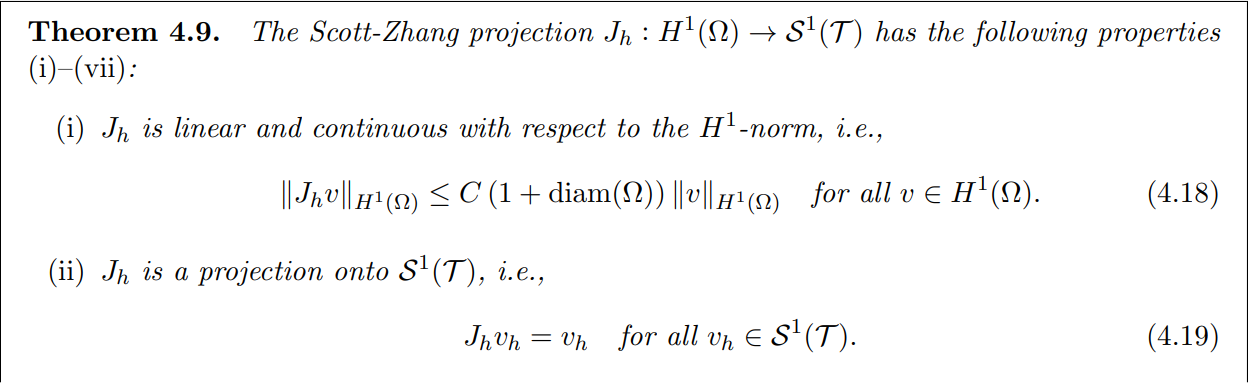
\includegraphics[width = 0.75 \textwidth]{NumPDEs/NumPDEs - Theorem 4.9.1.png} \\
    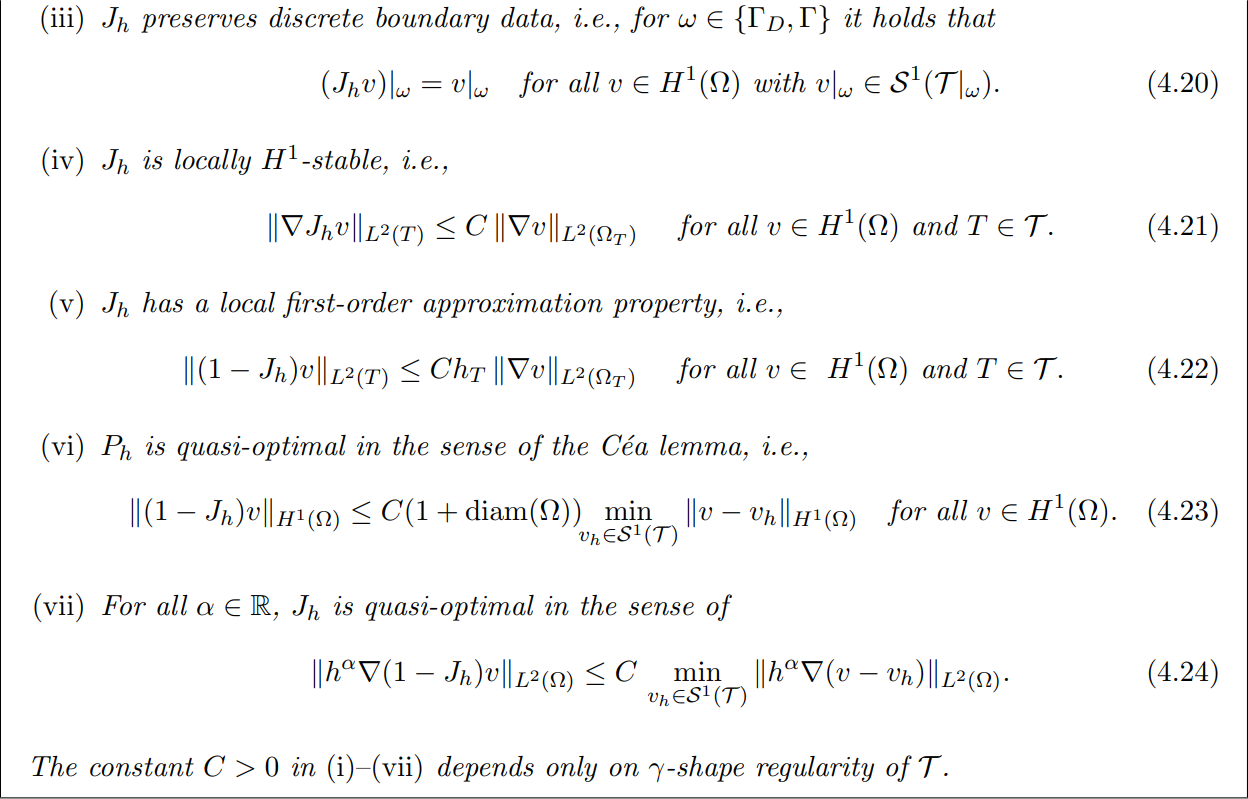
\includegraphics[width = 0.75 \textwidth]{NumPDEs/NumPDEs - Theorem 4.9.2.png}
  \end{tcolorbox}

  \begin{tcolorbox}[standard jigsaw, opacityback = 0]
    \centering
    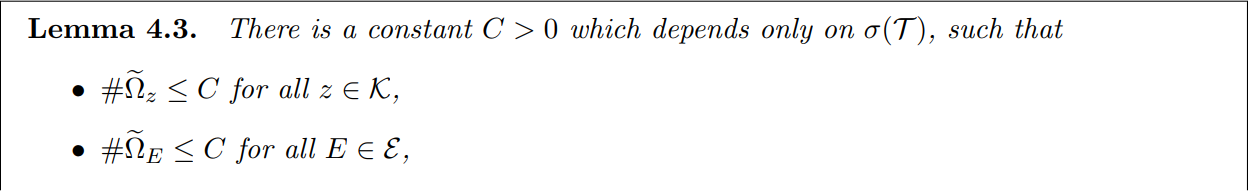
\includegraphics[width = 0.75 \textwidth]{NumPDEs/NumPDEs - Lemma 4.3.1.png} \\
    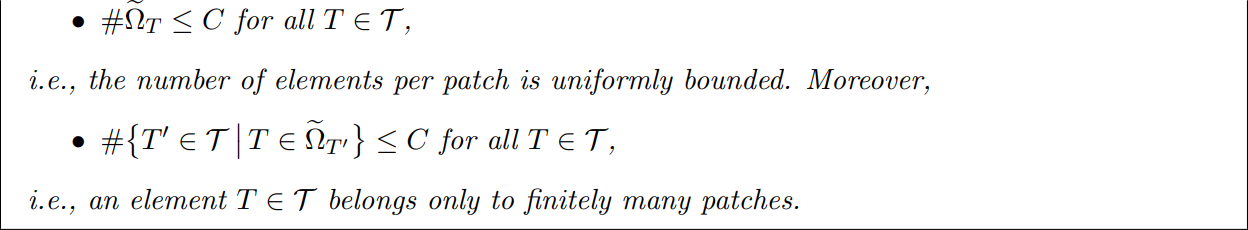
\includegraphics[width = 0.75 \textwidth]{NumPDEs/NumPDEs - Lemma 4.3.2.png}
  \end{tcolorbox}

  Die Approximations-Eigenschaft des Clément-Operators $J_h$, d.h. Lemma 4.9 (v) und der letzte Unterpunkt von Lemma 4.3 implizieren

  \begin{align*}
    & \sum_{T \in \mathcal{T}}
    \norm[L^2(T)]{f - (b \cdot \nabla u_h + c u_h)}
    \norm[L^2(T)]{v - J_h v} \\
    & \stackrel
    {
      \mathrm{4.9 (v)}
    }{\leq}
    \sum_{T \in \mathcal{T}}
    \norm[L^2(T)]{f - (b \cdot \nabla u_h + c u_h)}
    C_1 h_T
    \norm[L^2(\Omega_T)]{\nabla v} \\
    & \stackrel
    {
      \mathrm{CSB}
    }{\leq}
    C_1
    \pbraces
    {
      \sum_{T \in \mathcal{T}}
      \norm[L^2(T)]{h_\mathcal{T} (f - b \cdot \nabla u_h - c u_h)}^2
    }^{1/2}
    \pbraces
    {
      \sum_{T \in \mathcal{T}}
      \norm[L^2(\Omega_T)]{\nabla v}^2
    }^{1/2} \\
    & \stackrel
    {
      \mathrm{4.3}
    }{\leq}
    C_1 C_2
    \pbraces
    {
      \sum_{T \in \mathcal{T}}
      \norm[L^2(T)]{h_\mathcal{T} (f - b \cdot \nabla u_h - c u_h)}^2
    }^{1/2}
    \pbraces
    {
      \sum_{T \in \mathcal{T}}
      \norm[L^2(T)]{\nabla v}^2
    }^{1/2} \\
    & =
    C_1 C_2
    \norm[L^2(\Omega)]{h_\mathcal{T} (f - b \cdot \nabla u_h - c u_h)}
    \norm[L^2(\Omega)]{\nabla v}
  \end{align*}

  Für jede Kante $E \in \mathcal{E}$, wählen wir ein arbiträres Element $T_E \in \mathcal{T}$ mit $E \in \mathcal{E}_{T_E}$.
  Sei $\mathcal{E}_\ast \subset \mathcal{E}$ und $\psi \in L^2(E)$ für alle $E \in \mathcal{E}_\ast$.
  Man erinnere sich an Lemma 4.10.

  \includegraphicsboxed{NumPDEs/NumPDEs - Lemma 4.10.png}

  Daher, zeigen die selben Argumente wie zuvor, dass

  \begin{align*}
    \sum_{E \in \mathcal{E}_\ast}
    \norm[L^2(E)]{\psi}
    \norm[L^2(E)]{v - J_h v}
    & \stackrel
    {
      \mathrm{4.10}
    }{\leq}
    \sum_{E \in \mathcal{E}_\ast}
    \norm[L^2(E)]{\psi}
    C_3 h_E^{1/2}
    \norm[L^2(\Omega_{T_E})]{\nabla v} \\
    & \stackrel
    {
      \mathrm{CSB}
    }{\leq}
    C_3
    \pbraces
    {
      \sum_{E \in \mathcal{E}_\ast}
      \norm[L^2(E)]{h_\mathcal{E}^{1/2} \psi}^2
    }^{1/2}
    \pbraces
    {
      \sum_{E \in \mathcal{E}_\ast}
      \norm[L^2(\Omega_{T_E})]{\nabla v}^2
    }^{1/2} \\
    & \stackrel{!}{\leq}
    C_3
    \pbraces
    {
      \sum_{E \in \mathcal{E}_\ast}
      \norm[L^2(E)]{h_\mathcal{E}^{1/2} \psi}^2
    }^{1/2}
    \pbraces
    {
      3
      \sum_{T \in \mathcal{T}}
      \norm[L^2(T)]{\nabla v}^2
    }^{1/2} \\
    & =
    \sqrt{3} C_3
    \norm[L^2(\mathcal{E}_\ast)]{h_\mathcal{E}^{1/2} \psi}
    \norm[L^2(\Omega)]{\nabla v},
  \end{align*}

  wobei wir bemerken, dass ein Element $T \in \mathcal{T}$ nur $= T_E$ sein kann auf höchstens $3$ Kanten.
  Die Euklid-Norm ist zur Manhattan-Norm auf dem $\R^2$ äquivalent, vermöge $1$ bzw. $\sqrt{2}$.
  Insgesamt sehen wir nun ($\psi := \dbbraces{\partial_n u_h}$ und $\mathcal{E}_\ast := \mathcal{E}_\Omega)$)

  \begin{align*}
    R_h(v)
    & \leq
    C_1 C_2
    \norm[L^2(\Omega)]{h_\mathcal{T} (f - b \cdot \nabla u_h - c u_h)}
    \norm[L^2(\Omega)]{\nabla v}
    +
    \sqrt{3} C_3
    \norm[L^2(\mathcal{E}_\Omega)]{h_\mathcal{E}^{1/2} \dbbraces{\partial_n(A u_h)}}
    \norm[L^2(\Omega)]{\nabla v} \\
    & \leq
    \max \Bbraces{C_1 C_2, \sqrt{3} C_3}
    \norm[L^2(\Omega)]{\nabla v}
    \pbraces
    {
      \norm[L^2(\Omega)]{h_\mathcal{T} (f - b \cdot \nabla u_h - c u_h)}
      +
      \norm[L^2(\mathcal{E}_\Omega)]{h_\mathcal{E}^{1/2} \dbbraces{\partial_n (A u_h)}}
    } \\
    & \leq
    \max \Bbraces{C_1 C_2, \sqrt{3} C_3}
    \norm[L^2(\Omega)]{\nabla v}
    \sqrt{2}
    \pbraces
    {
      \norm[L^2(\Omega)]{h_\mathcal{T} (f - b \cdot \nabla u_h - c u_h)}^2
      +
      \norm[L^2(\mathcal{E}_\Omega)]{h_\mathcal{E}^{1/2} \dbbraces{\partial_n (A u_h)}}^2
    }^{1/2} \\
    & \leq
    \sqrt{2}
    \max \Bbraces{C_1 C_2, \sqrt{3} C_3}
    \norm[L^2(\Omega)]{\nabla v}
    \eta.
  \end{align*}

  Nun gilt es, die Vorbemerkungen des Beweises von dem originalem Theorem 4.11 nachzubauen.
  Weil $v \in H_D^1(\Omega)$ beliebig war, folgt

  \begin{align*}
    \implies
    \sup_{w \in H_D^1(\Omega) \setminus \{0\}}
    \frac
    {
      R_h(w)
    }{
      \norm[L^2(\Omega)]{\nabla w}
    }
    \leq
    \sqrt{2}
    \max \Bbraces{C_1 C_2, \sqrt{3} C_3}
    \eta.
  \end{align*}

  Nachdem $u \in H_D^1(\Omega)$ ja eine schwache Lösung ist,

  \begin{align*}
    \implies
    R_h(v)
    =
    F(v) - a(u_h, v)
    =
    \underbrace
    {
      F(v) - a(u, v)
    }_0
    +
    a(u, v)
    -
    a(u_h, v)
    =
    a(u - u_h, v).
  \end{align*}

  Es seien $L$ die Stetigkeits- und $M$ die Elliptizitäts-Konstante von $a$.

  \begin{multline*}
    M \norm[H^1(\Omega)]{u - u_h}
    =
    \frac
    {
      M \norm[H^1(\Omega)]{u - u_h}^2
    }{
      \norm[H^1(\Omega)]{u - u_h}
    }
    \leq
    \frac
    {
      M \norm[H^1(\Omega)]{u - u_h}^2
    }{
      \norm[L^2(\Omega)]{\nabla (u - u_h)}
    }
    \leq
    \frac
    {
      a(u - u_h, u - u_h)
    }{
      \norm[L^2(\Omega)]{\nabla (u - u_h)}
    } \\
    =
    \frac
    {
      R_h(u - u_h)
    }{
      \norm[L^2(\Omega)]{\nabla (u - u_h)}
    }
    \leq
    \sup_{w \in H_D^1(\Omega)}
    \frac
    {
      R_h(w)
    }{
      \norm[L^2(\Omega)]{\nabla w}
    }
  \end{multline*}

  Damit erhalten wir nun endlich unsere finale Abschätzung.

  \begin{align*}
    C
    :=
    \frac
    {
      \sqrt{2}
      \max \Bbraces{C_1 C_2, \sqrt{3} C_3}
    }{
      M
    }
    \implies
    \norm[H^1(\Omega)]{u - u_h}
    \leq
    C \eta
  \end{align*}

  Die (nicht versteckte) Konstante $C$ hängt nur ab (von dem Clemént-Operator $J_h$ und) von der $\gamma$-Form-Regularität von $\mathcal{T}$.

\end{enumerate}

\end{solution}

% --------------------------------------------------------------------------------
